\section{Introduction}
Recently, with the advancement of technology, a large cohort of studies are considering an automated computer-aided diagnosis of autism \cite{leo2019computational, han2017global, liu2017technology} and also developing interactive tools to aid in the rehabilitation and treatment of autistic patients \cite{johnston2020soundfields, johnston2019measuring, magrini2019augmented}. Such automated approaches would decrease subjectivity and improve diagnostic reproducibility and availability. It would also play a substantial role in ensuring early diagnosis. \\

The two most fundamental and widely used MRI image types are – 1) Structural (sometimes
called anatomical) and 2) Functional images. A structural MRI image is a three-dimensional
image that contains information about the anatomy of the brain like grey/white matter
volume, \Gls{CSF} (cerebrospinal fluid), etc. While functional MRI scans produce a set of 3D
images recorded over time and measure a signal (most commonly, the \gls{BOLD} signal) that is
related to neural activity. Magnetic resonance imaging (MRI) can be used to detect various neuropsychiatric and neurodegenerative disorders, such as schizophrenia \cite{garrity2007aberrant, zhou2007functional, jafri2008method, calhoun2012exploring}, dementia, depression \cite{craddock2009disease}, autism \cite{plitt2015functional, anderson2011functional, shi2020fmri, rakhimberdina2020population}, ADHD \cite{zhang2020separated}, Alzheimer’s \cite{greicius2004default, chen2011classification}, etc., by observing anatomical patterns of the brain using structural MRI data or by connecting changes in the brains’ functional architecture to psychiatric health conditions using functional MRI data.\\

Since this research work deals only with autism detection, the focus of this chapter is to
present a comprehensive literature review of various ASD detection approaches using either
structural and functional MRI and a combined approach that includes both. In this regard,
functional MRI indicates only resting-state functional MRI i.e, rs-fMRI. Through providing a
summary of previous related studies, this part of the thesis discusses methods applied by
different researchers, their performance evaluation, challenges faced and limitations. A brief overview of fMRI is also represented in the following section in order to familiarize with the type of data generated by fMRI scans.\\

\section{Overview of Functional Magnetic Resonance Imaging (fMRI)}
A human brain can be defined as a complex agglomeration of interconnected systems
comprising a large number of regions conducting various functions. Although some structural
regions may not possess unmediated and direct connection, they are associated globally to
process numerous varieties of information as a whole \cite{guo2017diagnosing}. Magnetic Resonance Imaging or
MRI is a radiological technique used to visualize 3D images representing the anatomical and
physiological processes of the brain \cite{wikipedia_2021}. Functional MRI or fMRI is a special type of MRI that
measures spontaneous fluctuations in brain activity by detecting changes related to blood
using the BOLD signal while the subject performs an explicit task such as, tapping his/her
finger, moving his/her arm, squeezing a ball, looking at a picture, etc.\\

BOLD is the abbreviation for Blood Oxygen Level Dependent. It is a time-varying signal
modulated by changes in the oxygen content of the blood that enables in identifying active
brain areas while performing a task. Neurons in the active brain areas that respond in carrying
out the task tend to receive a high amount of oxygenated blood which in turn increases the
BOLD signal intensity measured in that area. A human brain is a 3D object and fMRI takes
picture of it by making a series of slices and within each slice there exists a 2D picture of
neuronal activities going on in that slice. Such 3D images are taken at different timepoints
recording the change of activities across time. Thus a raw fMRI data of a single subject is 4D
where the 4th dimension represents time.\\

\begin{figure}[h]
\centering
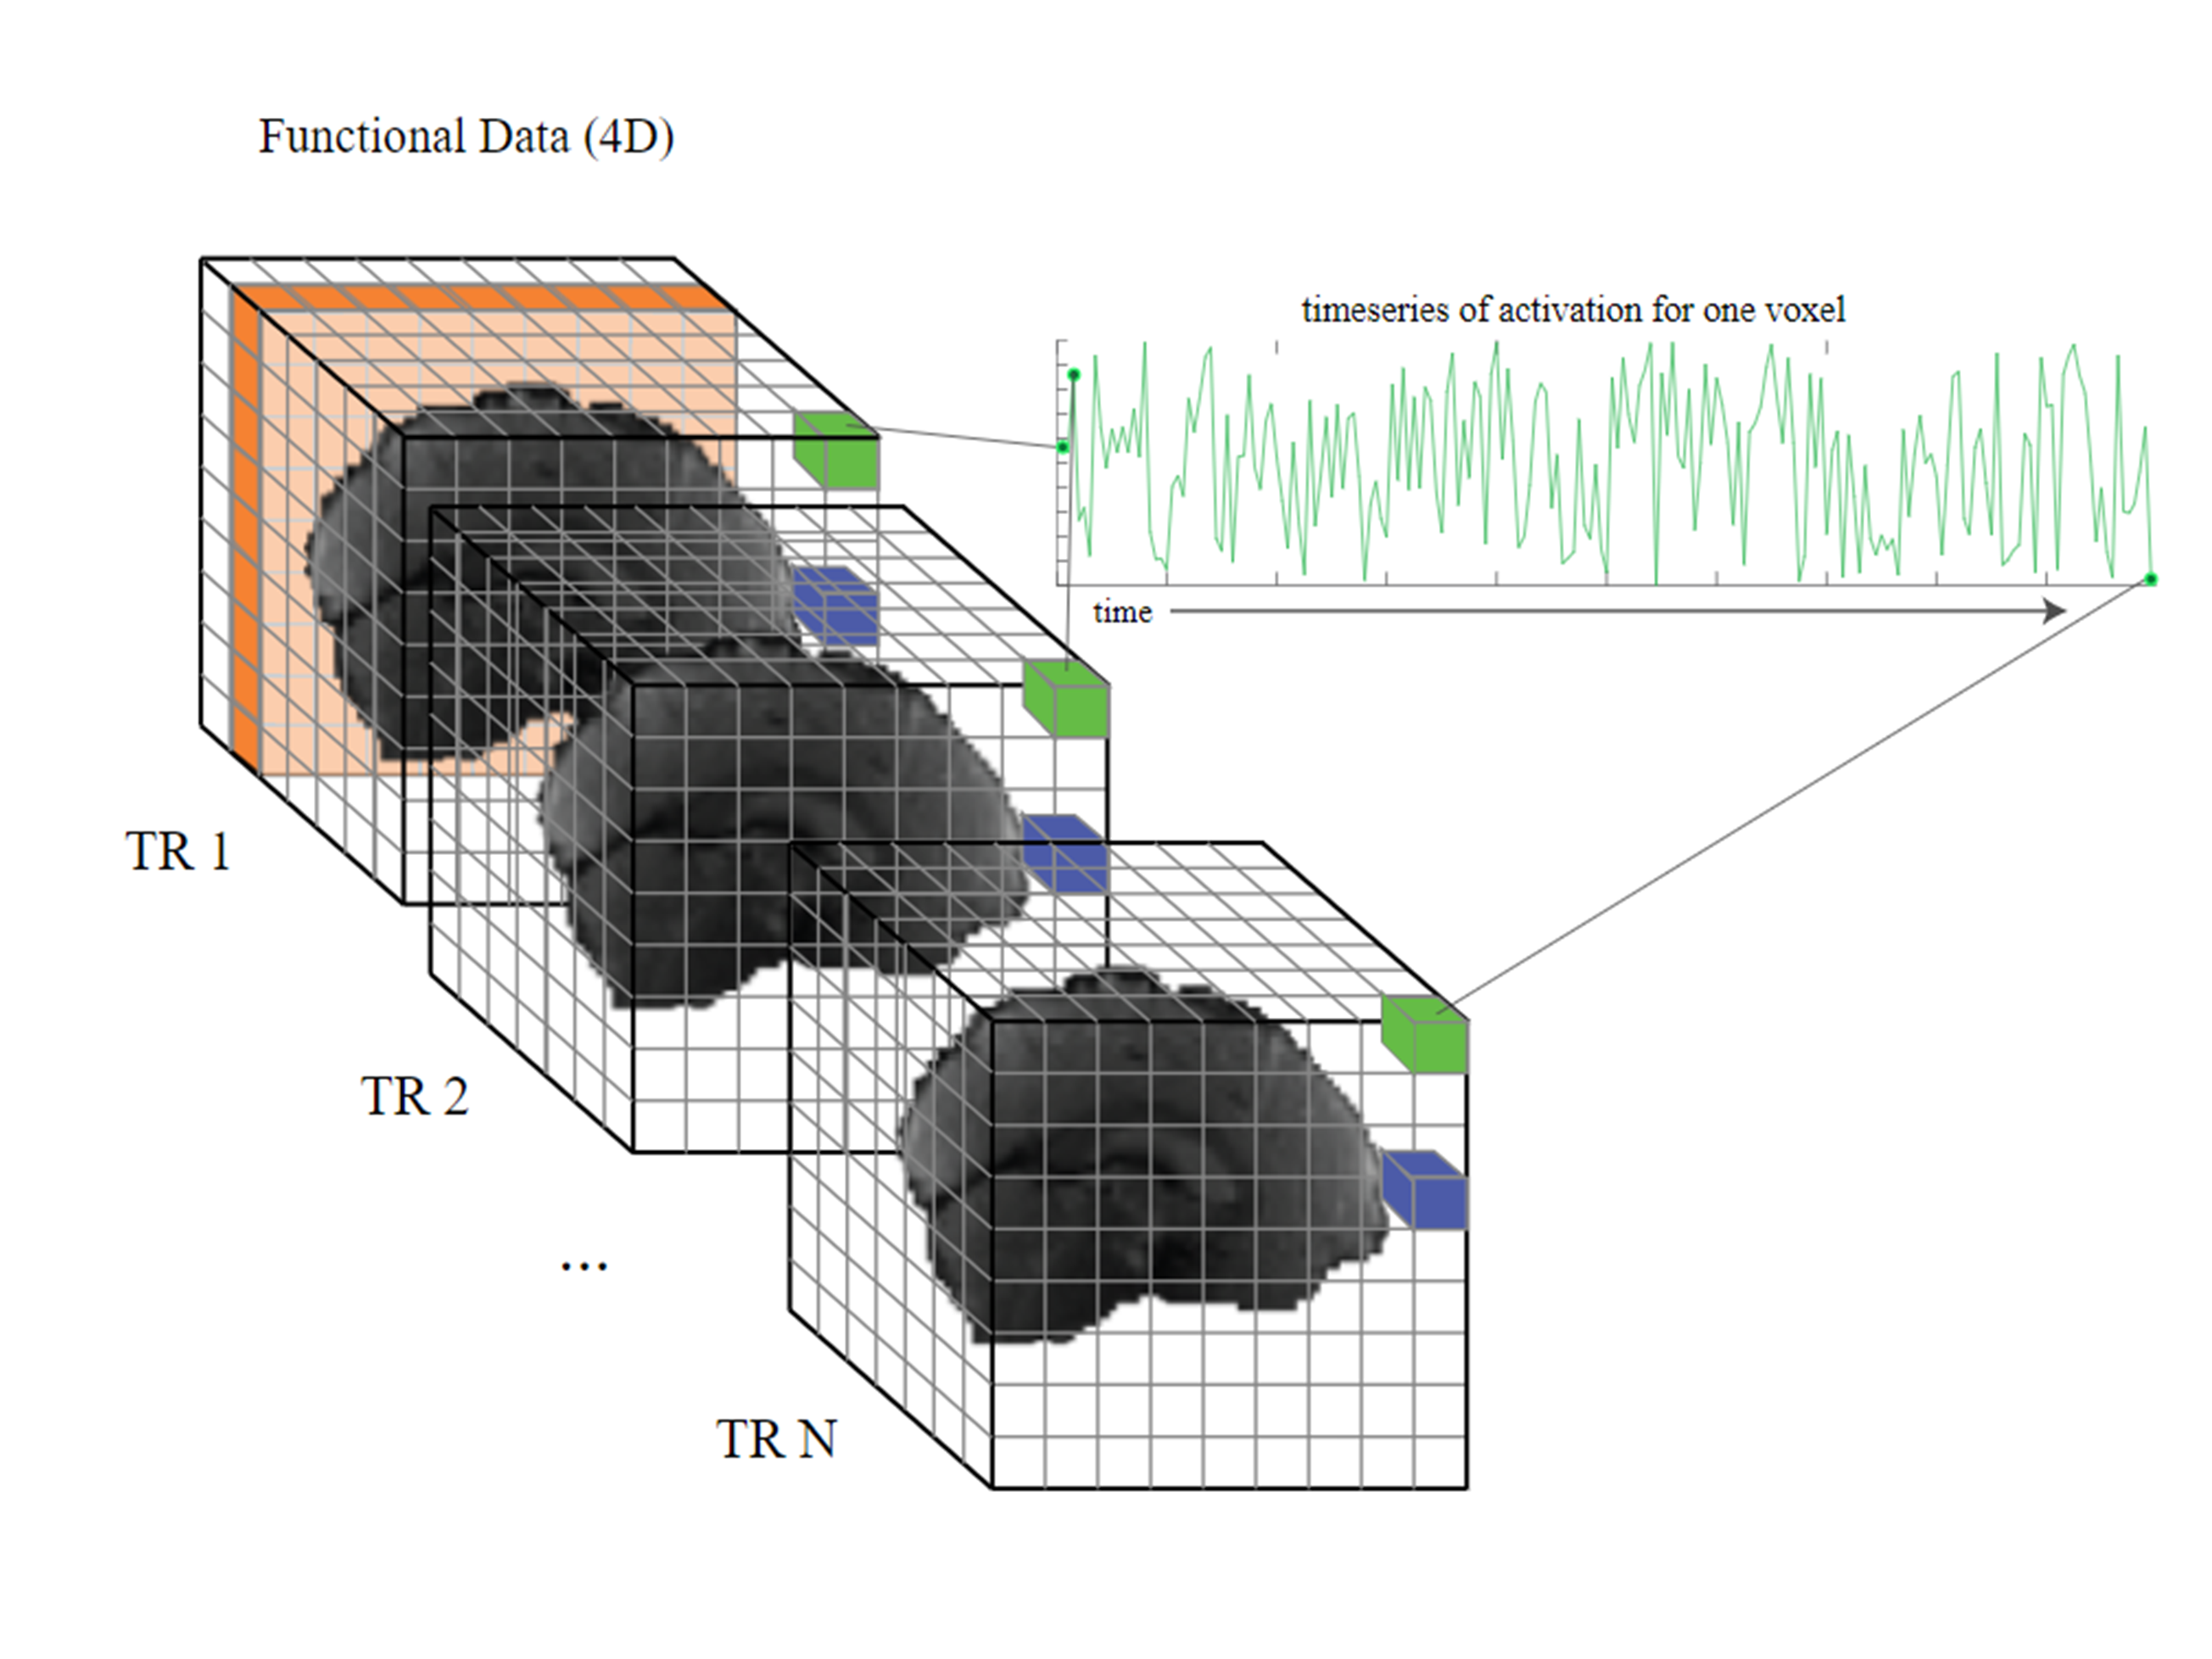
\includegraphics[width=\textwidth]{figures/2.1 overview of fMRI.png}
\caption{Representation of fMRI data.}
\label{fig: 2.1}
\end{figure}

Some basic terminologies related to fMRI data are discussed:\\

\begin{itemize}
\item \textbf{Volume:} The entire three-dimensional pixel grid covering the space that was imaged
by the MRI scanner. The volume is composed of many smaller voxels. Functional
data has a volume for each time point of the experiment.
\item \textbf{Voxel:} A three-dimensional pixel and the basic unit of spatial measurement in MRI
(represented by green and blue cubes in Figure \ref{fig: 2.1}).
\item \textbf{Slice:} All of the voxels in a 2D plane taken from the 3D volume (shown in orange in
Figure \ref{fig: 2.1}).
\item \textbf{TR:} Abbreviation for repetition time. The basic unit of time in functional MRI.
One volume is scanned every TR.
\end{itemize}

Resting-state fMRI (rs-fMRI) is a special type of f-MRI technique that performs brain
mapping to evaluate regional interactions occurring in a task-negative state i.e when an
explicit task is not being performed. In this case, a subject lies in the MRI scanner without
thinking or doing anything in particular according to \cite{biswal2012resting}. The data utilized in this study is
resting-state fMRI data which is devoid of the complications and difficulties associated with
task-evoked or fMRI data.


\section{Related Literature Review}
\subsection{Detection using Structural MRI (sMRI)}
Structural MRI studies emphasise upon volumetric and morphometric analyses to detect
abnormal brain anatomy.\\

A voxel-based morphometry analysis was performed by Riddle et al. in \cite{riddle2017brain} and it was
observed that the grey matter volumes, the left anterior superior temporal gyrus and the total
brain volume are enlarged in ASD children by 1-2\% approximately.\\

Besides, Aylward et al. in \cite{aylward2002effects} measured total brain volumes and head circumference from
1.5-mm coronal MRI scans in 67 autistic subjects and 83 healthy community volunteers
within the age range of 8-46 years but observed no brain volumetric differences between
ASD and control subjects aged above 12. Thus, total brain volume cannot be treated as a
biomarker to detect ASD comprising all age range.\\

Palmen et al. in \cite{palmen2005increased} acquired brain MRI scans from 21 high-functioning autistic subjects and
21 control subjects belonging to 7-15 years. This study concluded that high-functioning
autistic subjects showed an enlargement of grey-matter volume. No increase in white-matter
and cerebellar volume was observed. However, Courchesne et al. in \cite{courchesne2007mapping} also reported an
increase in grey matter volume, particularly in the temporal lobes in autism.\\

On the contrary, an increased white matter and reduced cerebral cortex and hippocampusamygdala
were found in the autistic brain by Herbert et al. \cite{herbert2003dissociations} performing MRI-based
morphometric analysis on all-male subjects that included 17 autistic and 15 control ones
between 7-11 years of age. Conversely, Jou et al. in \cite{jou2011reduced} observed decreased central white
matter volume in autistic subjects performing experiments using MRI data obtained at 1.5-T
and analyzed via BRAINS2 software from 23 autistic and 23 matched control boys.\\

Thus, all the previous works of literature stated above failed to reach strong conclusions
regarding volumetric changes using only structural MRI data and presented inconsistent
findings regarding grey and white matter volumes in autism and control brain. The use of
small sample size, limited age range and including only male subjects can be regarded as a
limitation.\\

However, Kong et al. in \cite{kong2019classification} presented a promising study and a unique methodology to solve
the classification problem using structural information from MRI data. An individual brain
network was constructed for each subject and connectivity features were extracted between
each pair of ROIs. Then, these features were ranked by Fisher score computation. The top
3000 features were provided as input to a deep neural network classifier. Results showed a
very high accuracy of 90.39\% and an AUC score of 97.38\% using 182 subjects from a single
site. However, such low number of participants might result in poor generalization.\\

\subsection{Detection using resting-state functional MRI (rs-MRI)}
Biswal et al. in \cite{biswal1995functional} discovered that different brain regions actively interact with each
other while a subject was at rest i.e, not performing any cognitive task. Then onwards, rsfMRI
has evolved as a noteworthy tool to explore brain networks by investigating local and
global connectivity patterns. At present, it is recognized as one of the most efficient methods
to detect different brain disorders.\\

Nielson et al. in \cite{nielsen2013multisite} used whole-brain point-to-point functional connectivity including rsfMRI
data obtained from the ABIDE (Autism Brain Imaging Data Exchange) dataset
comprising 964 subjects collected from 16 different international sites. Raw image data were
preprocessed in MATLAB using SP8. After preprocessing, mean BOLD signals for each
subject were extracted from 7266 grey matter ROIs. A 7266×7266 association matrix
representing functional connectivity between every ROI pairs was computed from Pearson
correlation coefficients for every subject. Each ROI pairs were defined as a connection.
Connections, categorized into several bins and a general linear model classifier was fitted on
bins containing connections. Very low accuracy of merely 60\% was achieved for whole-brain
classification.

Heinsfeld et al. \cite{heinsfeld2018identification} applied deep learning algorithm combining a multilayered perceptron
(MLP) along with the unsupervised training of two stacked denoising autoencoders. Here,
preprocessed data were downloaded from the CPAC preprocessing pipeline. Mean time series
was extracted using the CC200 ROI atlas for each subject. Time series for each subject was
converted to a 200×200 connectivity matrix using Pearson correlation coefficient which was
further reduced to a feature vector comprising 19,900 features by removing the upper half
triangular part and principal diagonal from the connectivity matrix. The remaining lower
triangular part was flattened to a feature vector containing derived features from MRI image
data and finally fed to the deep learning classifier. 70\% mean classification accuracy was obtained and brain areas that contributed the most to classifying ASD and control were
identified. However, took a huge training time (over 32 hours).\\

Eslami et al. \cite{eslami2019asd} proposed ASD-Diagnet, a framework for detecting ASD using only rs-fMRI
data. A combined learning procedure using an autoencoder and a single layered perceptron
(SLP) was used which resulted in a greater quality of extracted features and optimized
parameters for the model in \cite{eslami2019asd}. Furthermore, to increase the number of training subjects a
data augmentation strategy, based on linear interpolation on available feature vectors was
implemented. However, this strategy could improve accuracy only by 1\% and presented a
mean classification accuracy of 70.1\%. It also gave an enormous advantage in the case of
training time (40 minutes).\\

A deep multimodal model able to learn a joint representation from 2 types of connectomic
data, (i) ROI time series activation map and (ii) fMRI×ROI activation map offered by rsfMRI
scans was proposed by Tang et al. in \cite{tang2020deep}. A 3D Resnet and MLP classifier were used
in the classification process. This approach displayed 74\% classification accuracy, 95\%
recall, 0.805 F1-score and proved an overall superior performance using a single type of
functional data.\\

\subsection{Detection in a Combined Approach using both sMRI and rs-fMRI}
A fusion approach using both structural and functional data have also been applied in the
ASD and control classification pipeline. Each element in a functional data-based connectivity
matrix imparts information regarding correlation coefficients of averaged BOLD signal from
ROI pairs. On the contrary, elements in a structural data-based connectivity matrix provide
information regarding cortical grey matter volumes.\\

Rakić et al. \cite{rakic2020improving} proposed such a combined approach using 817 cases from the \Gls{ABIDE}
dataset. Steps of the framework included preprocessing structural (using FreeSurfer software)
and functional (\Gls{CPAC} preprocessing pipeline) data, feature extraction (using \Gls{AAL} and
\Gls{CC200} parcellation for functional and Destrieux atlas for structural data) and representation
using connectivity matrices. Fisher score was computed for feature reduction and finally, data
classification was performed by an ensemble of autoencoders and \Gls{MLP} 85.06 ± 3.52\%
classification accuracy was obtained using an ensemble of classifiers.\\

The research conducted by Mellema et al. in \cite{mellema2019multiple} compared classification performance via 12
classifiers using more than 900 subjects from the \Gls{IMPAC} database. The derived structural and functional features were obtained directly from IMPAC. The 12 classifiers included 6
nonlinear shallow models, 3 linear shallow models and 3 deep learning model. For structural
data, the Desikan-Killiany gyrus atlas was used to extract ROIs. While functional data used 7
different predefined atlases namely: \Gls{BASC}-64, BASC-122, BASC-197, Craddock which
defines 249 ROIs, Harvard-Oxford containing 69 ROIs, \Gls{MSDL} with 39 ROIs and the Power
Atlas comprising 264 ROIs. For connectivity matrix parametrization, tangent space
embedding was used. The dense FeedFWD network was found to be the best model
achieving 0.80 \Gls{AUC} with the fusion of anatomical data and functional data from \Gls{BASC} atlas
comprising 122 ROIs.\\

\section{Conclusion}
In this chapter, a detailed literature review of related works has been discussed. For
convenience, this discussion was divided into three categories depending on the proposed
approach and data type used. From the above discussion, it is evident that structural MRI
data approaches mainly focused on determining common brain patterns between ASD vs
control rather than solving the inherent classification problem. Structural data-based studies
also resulted in inconsistent findings. On the contrary, combined approaches resulted in quite
satisfactory results but it requires the availability of both types of MRI data for each patient
which might be problematic in a practical scenario. Thus, in this study, we will mainly focus
on improving the existing classification accuracy using only rs-fMRI data. An elaborate
description of the proposed methodology will be discussed in the upcoming chapter.

\subsection{Implementation Challenges}
The implementation of this research work posed a number of challenges which are stated:\\

\begin{itemize}
    \item \textbf{Optimizing a massive number of parameters:} In this thesis, we used a deep neural
network classifier. Such deep learning-based classifiers require optimizing a massive
amount of hyperparameters such as hidden layer configuration, neurons per layer,
regularization technique, activation function, amount of dropout, etc. Especially high
dimensional dataset and limited training samples (which is the case in the
neuroscientific community) make the task of hyperparameter searching, optimization
and overfitting prevention even more strenuous.

\item \textbf{Difficulties in detection without demographic information:} Various studies used
the demographic information of the subjects such as age, IQ, and handedness in their
methods or selected subsets of subjects with specific attributes in their analysis in \cite{eslami2019asd}
However, using only fMRI data without taking into account other phenotypic and
demographic information would ensure an independent and unbiased decision in
diagnosis. Although, the presence of such demographic information would result in
higher predictive power. But, our objective is to depend solely on fMRI data to avoid
biases, which is a more challenging task.
\end{itemize}